% Number 590
% UFPM  Inclines CAPMA CAPMG Algebra Units 
% Cart sliding up incline
% JG

% Watermark
\AddToShipoutPicture*{\BackgroundPic}

\addtocounter {ProbNum} {1}

%\begin{floatingfigure}[r]{.2\textwidth}
%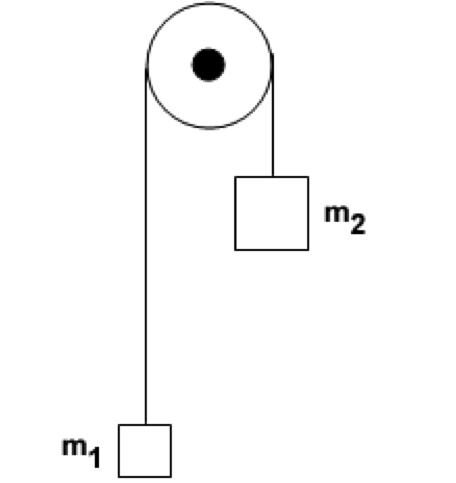
\includegraphics[scale=.8]{/Users/jgates/desktop/latex/pics/Atwood3}
%\end{floatingfigure}
 
{\bf \Large{\arabic{ProbNum}}} A glider is given a quick push to start it moving up a ${7^{\circ}}$ inlined air track. The glider travels to a maximum distance of 112 cm up the track.

\bigskip
Determine the initial speed of the glider.
 
\vfill
\vfill

Draw a velocity graph for the glider; use the graph to determine how long the glider takes to get to that 112 cm point.
\vfill

Use your velocity graph to determine where the glider will be 2 seconds after it was launched.
\vspace{30 mm}
%\hfill 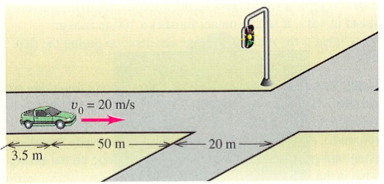
\includegraphics[scale=.85]{/Users/jgates/desktop/latex/pics/redlight.png}
\newpage